% Chapter 1
% 
\chapter{Introduction} % Main chapter title
\label{chap:Chapter1} % For referencing the chapter elsewhere, use Chapter~\ref{Chapter1}


%-------------------------------------------------------------------------------
%---------
%
\section{Context} 


\section{Problem}

A Natixis é uma empresa do setor financeiro, parte do grupo bancário francês BPCE (Banque Populaire,
 Caisse d'Epargne). Ela atua principalmente em banca de investimentos, gestão de ativos, seguros e serviços
 financeiros especializados [1].

 Atualmente a equipa "B2C" da Natixis efetua tarefas diárias de suporte técnico no sistema pelo qual é
 responsável. Este é um sistema maioritariamente responsável pelo cálculo de risco de crédito bancário. O
 sistema respeita um fluxo bem definido sendo que diariamente correm diversos processos. Primeiramente
 vem a fase de alimentação, onde o sistema injeta dados provenientes de sistemas externos e popula as
 tabelas brutas da base de dados. De seguida vem o processo de enriquecimento dos dados, onde os
 mesmos são analisados em termos de qualidade, sendo aplicadas regras de negócio para os alterar e
 armazenar. Todo esse processo é auditado em ficheiros e/ou tabelas específicas na base de dados. Por fim
 vem o processo de cálculo, que pode ser de vários tipos, como por exemplo RC B3 (Cálculo do Capital
 Ponderado pelo Risco - B3) que nos sistemas bancários se refere, normalmente, aos requisitos de capital
 regulamentares definidos pelo acordo de Basel III [2].
 Todo este processo é controlado diariamente pelo Control-M. O Control-M é uma ferramenta de automação
 de workload e gestão de jobs [3]. Ele é amplamente utilizado para agendar, monitorizar e gerir processos
 batch. A equipa de suporte é responsável por gerir esta chain, sendo que cada processo (alimentação,
 enriquecimento e cálculo) é composto por diversos batchs que executam maioritariamente código Perl e
 Java.

 Falhas na chain são comuns de acontecer e podem ter diversos motivos, como erros nos dados externos que
 violem as regras de negócio, problemas de código provenientes de desenvolvimentos recentes, entre outros.
 A equipa é também responsável por lançar processos "on demand", facilitar o esclarecimento de questões
 relacionadas com regras de negócio aos utilizadores/partes interessadas, entre outras atividades.
 Devido à dimensão do software e à quantidade de diferentes processos envolvidos, por vezes a atividade de
 suporte torna-se uma tarefa bastante complicada para a equipa responsável.



\section{Objectives}

Explorar Retrieval-augmented generation (RAG) juntamente com Large Language Model (LLM) para construir
 um sistema que forneça auxílio à tomada de decisão nas atividades de suporte, pela geração de informação
 contextualizada.
 Retrieval-Augmented Generation (RAG) combina a geração de texto por Large Language Models (LLMs) com
 recuperação de conhecimento externo, permitindo respostas mais informadas e específicas [4].
 Os LLMs, como GPT, Llama e Mistral, são modelos que possuem um vasto conhecimento, mas não
 conseguem aceder a informações de domínios específicos. O RAG resolve essa limitação ao combinar uma
 base de dados vetorial para armazenar representações semânticas de documentos e consultas, permitindo
 que o modelo recupere a informação mais relevante antes de gerar uma resposta. Essas bases de dados
 vetoriais utilizam embeddings, que representam o significado semântico do texto em um espaço
 multidimensional, possibilitando pesquisas mais eficientes e contextuais [4,5].
 A aplicação do RAG neste contexto permitirá otimizar a eficiência da equipa de suporte, reduzindo o tempo
 gasto na procura de informação e facilitando a resolução de incidentes.

 Funcionalidades a explorar:

 - Facilitar e agilizar a obtenção de informação relevante para resolução de determinado problema. O
 software deverá fornecer insights de passos a tomar com base no conhecimento que possui.
 - Automatizar a extração de conhecimento de fontes diversas, como manuais e logs de execução,
 integrando-se com as ferramentas utilizadas pela equipa (p.e. Control-M, Confluence, Outlook e Teams).
 - Auxiliar na resolução de problemas ao sugerir soluções com base em experiências anteriores e na
 análise de padrões de erro.

 O projeto irá obedecer à seguinte ordem cronológica:

 - Primeira fase: Análise de KPIs históricos na vertente de resolução de incidentes.
 - Segunda fase: Pesquisa / análise de trabalhos relacionados e boas práticas.
 - Terceira fase: Levantamento de requisitos.
 - Quarta fase: Implementação da solução.
 - Quinta fase: Testes.

\section{Metodologia}


A metodologia Design Science Research (DSR) (Figura \ref{fig:dsr}) foi escolhida como quadro orientador para o desenvolvimento deste trabalho. Esta metodologia é particularmente adequada para investigações que visam resolver problemas do mundo real através da criação e avaliação de artefactos inovadores (\cite{peffers2007design}).

\begin{figure}[H]
\centering
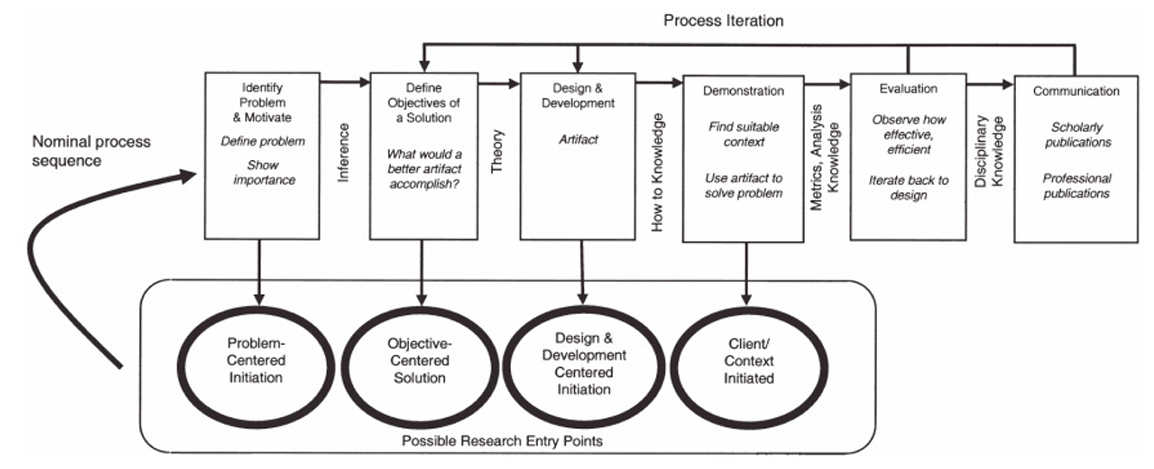
\includegraphics[width=1\linewidth]{ch1/dsr.png}
\caption{Metodologia DSR (\cite{peffers2007design})}
\label{fig:dsr}
\end{figure}

A metodologia DSR é composta por seis etapas, que se relacionam com o presente projeto da seguinte forma:

TODO retificar esta lista no fim do trabalho

\begin{itemize}
\item \textbf{Identificação e Motivação do Problema:} Foi realizada uma análise aprofundada dos desafios enfrentados pelas equipas de suporte técnico, nomeadamente a dificuldade em aceder rapidamente a informação precisa, a sobrecarga de pedidos repetitivos e a falta de padronização nas respostas.
\item \textbf{Definição de Objetivos para a Solução:} Com base nos problemas identificados, foram definidos objetivos claros, como a criação de uma solução baseada em RAG que melhore a eficiência do suporte técnico, assegure consistência nas respostas e possibilite a rastreabilidade das fontes de informação utilizadas.

\item \textbf{Desenho e Desenvolvimento:} Foi desenvolvido um protótipo funcional que integra uma arquitetura baseada em *Retrieval-Augmented Generation* com uma LLM, utilizando Spring AI. Este protótipo inclui também uma interface simples para interação e teste por parte dos utilizadores de suporte.

\item \textbf{Demonstração:} A solução foi aplicada a cenários simulados e reais de suporte técnico na área financeira, permitindo validar a sua aplicabilidade em tarefas como a resposta a incidentes, esclarecimento de dúvidas técnicas e recuperação de documentação normativa.

\item \textbf{Avaliação:} O sistema foi avaliado com base em testes de desempenho, testes unitários e de integração, bem como critérios de utilidade, precisão e conformidade com os requisitos regulatórios aplicáveis, incluindo os definidos pelo Banco Central Europeu.

\item \textbf{Comunicação:} Os resultados desta investigação foram documentados nesta dissertação e visam contribuir tanto para o avanço do conhecimento académico na área da IA aplicada ao suporte, como para a melhoria contínua de processos em contexto empresarial.

\end{itemize}




\section{Planeamento}


\section{Considerações Éticas}

Esta dissertação respeita o código de ética do Instituto Politécnico do Porto (\cite{codigo_2020}). Em conformidade com o Artigo 2.º, o trabalho observa princípios fundamentais como a legalidade, transparência, responsabilidade, confidencialidade, integridade e honestidade. Adicionalmente, a investigação cumpre as orientações previstas no Artigo 10.º, assegurando os mais elevados padrões de integridade científica, originalidade e verificabilidade.

O plágio e qualquer forma de má conduta académica são rigorosamente evitados, conforme estipulado no Artigo 6.º, nomeadamente na alínea 2.8, que exige a correta citação de todas as fontes. Quaisquer contributos de terceiros ou propriedade intelectual são devidamente creditados, em conformidade com o Artigo 10.º, alínea \textit{e}, que reforça a importância da citação precisa e da distinção relativamente a trabalhos anteriores.

Dado o carácter experimental desta investigação, apenas são utilizados conjuntos de dados e ferramentas com licenciamento explícito que permita a sua utilização académica. Além disso, e de acordo com o Artigo 10.º, alínea \textit{h}, eventuais conflitos de interesse e apoios externos são divulgados de forma transparente.

O conteúdo desta dissertação foi desenvolvido com diligência e rigor, garantindo a reprodutibilidade e a comunicação transparente dos resultados, conforme exigido pelo Artigo 10.º, alínea \textit{g}. Todos os métodos, fontes de dados e ferramentas utilizados nesta dissertação estão totalmente documentados e são publicamente acessíveis, contribuindo assim para uma comunicação científica aberta e transparente.

Por fim, todas as atividades foram realizadas com o devido respeito pelas obrigações éticas e legais no que respeita à privacidade de dados e à propriedade intelectual, conforme estipulado no Artigo 10.º, alínea 2a, e no Artigo 9.º, assegurando a segurança, bem-estar e os direitos de todos os participantes envolvidos.

\section{Estrutura do Documento}

